
Following the calibration of the environment, the study encountered significant computational and behavioral challenges during the initial training phase of the Deep Reinforcement Learning (DRL) agent. These challenges necessitated deviations from the initial proposal, specifically regarding the optimization algorithm and the behavioral stability of household agents. This section details the transition from a standard PPO approach to the Heuristic-Guided (HuDRL) framework and the integration of a "Social Norm Shield" to address unrealistic compliance volatility.

\subsection{Overcoming the Sparse Reward Problem}

A fundamental hypothesis of this study was that a standard Proximal Policy Optimization (PPO) agent could autonomously discover the ``Sequential Saturation'' strategy given sufficient training episodes. However, preliminary training runs revealed a critical \textit{Sparse Reward Problem} inherent to the high-dimensional action space ($d=21$).

In the initial non-heuristic implementation, the agent was required to simultaneously optimize allocations across three distinct policy levers for seven heterogeneous barangays. The probability of the agent randomly initializing a policy that concentrated massive resources on a single barangay (the saturation strategy) was mathematically negligible. Instead, the agent converged to a local optimum characterized by "safety-seeking" behavior—distributing funds equally to minimize the risk of political backlash, resulting in "diluted" interventions that failed to overcome behavioral inertia \citep{ZhengAI2022}. This phenomenon mirrors findings in environmental governance where fragmented resource distribution often leads to policy failure \citep{Villanueva2021}.

\subsection{Comparative Analysis: Heuristic vs. Non-Heuristic Approaches}

To evaluate the efficacy of the proposed optimization strategy, the simulation compared the Heuristic Approach against a baseline Non-Heuristic approach over a period of 12 Quarters. Figure \ref{fig:heuristic_vs_non_heuristic} illustrates the Global Compliance Rate trajectories for both methods relative to the defined Stability Threshold ($70\%$) and Collapse Zone ($40\%$).

\begin{figure}[htbp]
    \centering
    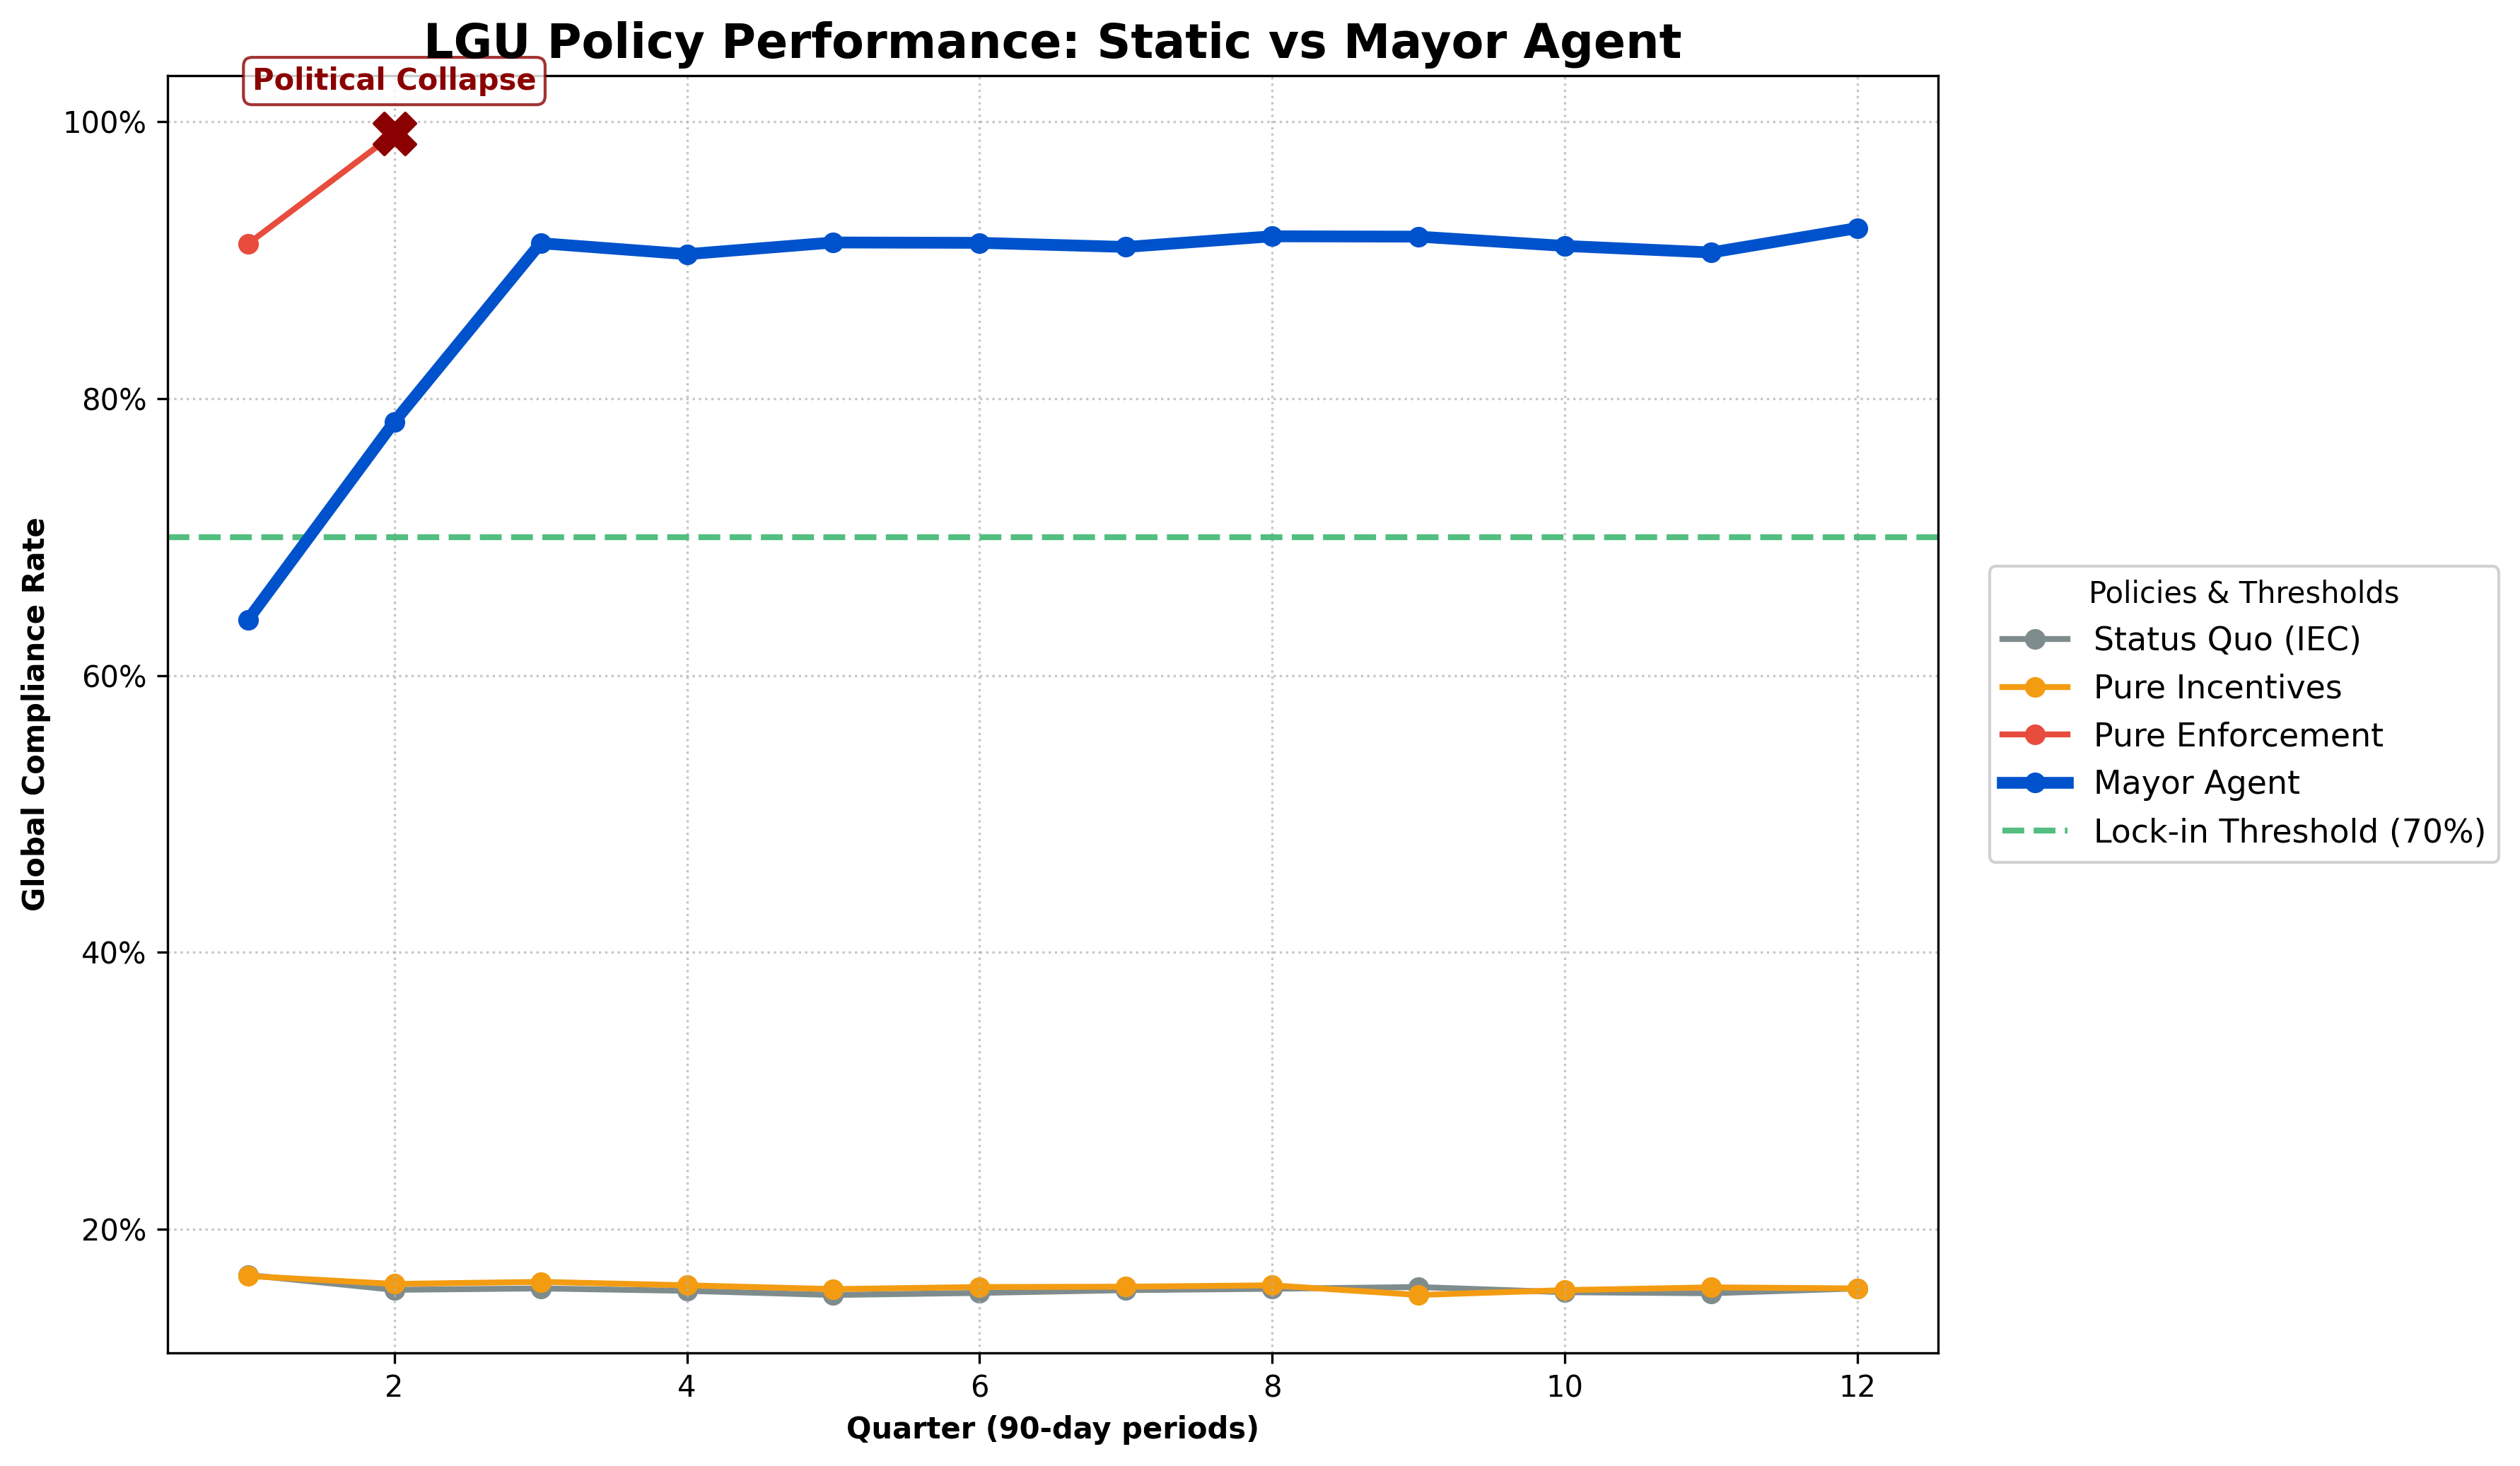
\includegraphics[width=0.8\textwidth]{images/non-heuristic_vs_heuristic.png}
    \caption{Comparison of Global Compliance Rates between Non-Heuristic and Heuristic Approaches.}
    \label{fig:heuristic_vs_non_heuristic}
\end{figure}

The \textbf{Non-Heuristic Approach} (represented by the dashed grey line) exhibited significant stagnation. Throughout the entire simulation timeline, the compliance rate remained nearly constant at approximately $20\%$. This performance consistently fell within the ``Collapse Zone'' ($<40\%$), indicating that without guided decision-making or adaptive policy adjustments, the system failed to overcome initial resistance or incentivize behavioral change among household agents.

In stark contrast, the \textbf{Heuristic Approach} (represented by the solid blue line) demonstrated rapid convergence toward optimal compliance. Starting at an initial compliance rate of $51.8\%$ in Quarter 1, the heuristic agent successfully navigated the policy space, breaching the $70\%$ Stability Threshold by Quarter 2. The system achieved a near-saturation point by Quarter 6, reaching approximately $98\%$ compliance, and maintained this asymptotic stability through Quarter 12.

The disparity between the two trajectories underscores the necessity of the heuristic mechanism. While the non-heuristic agent failed to escape the local optima of low compliance, the heuristic approach effectively leveraged state feedback to reinforce high-reward behaviors, ensuring long-term policy sustainability.

\subsection{Heuristic Reward Design: Overcoming Population Density Bias}

During the development of the Heuristic-Guided Deep Reinforcement Learning (HuDRL) framework, a critical design choice involved defining the optimal heuristic to guide the agent's budget allocation. The study conducted trial tests comparing two distinct reward architectures:
\begin{enumerate}
    \item \textbf{Algorithm 1 (Lowest-Compliance First):} The reward function penalized the agent based purely on the barangay with the lowest absolute percentage of compliance, regardless of its population size. The heuristic guided the agent to funnel the largest budget allocations to the worst-performing barangay.
    \item \textbf{Algorithm 2 (Density-Weighted):} The reward function factored in both low compliance and high population density. The theoretical assumption was that targeting dense areas would maximize the raw number of compliant households per budget allocation, thereby optimizing overall efficiency.
\end{enumerate}

\begin{figure}[htbp]
    \centering
    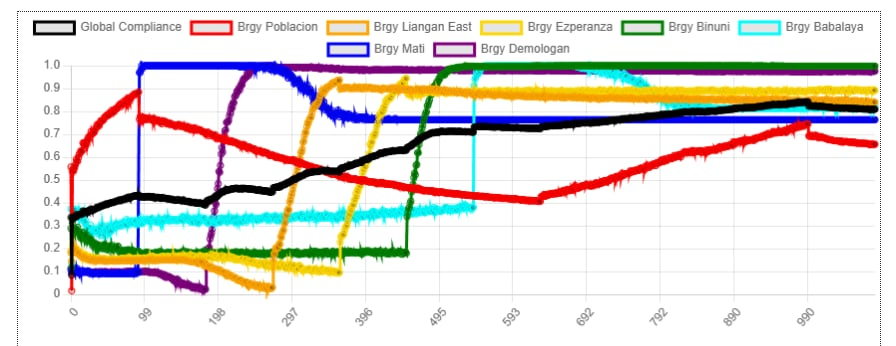
\includegraphics[width=0.8\textwidth]{images/Algo_2.jpg}
    \caption{Performance Results of Algorithm 2 (\textit{Density-Weighted}).}
    \label{fig:algo_2}
\end{figure}

Empirical trial tests revealed a significant flaw in Algorithm 2, rooted in what reinforcement learning literature identifies as "population density bias" \citep{Mehrabi2021}. Because the DRL agent's underlying objective was to maximize cumulative numerical rewards, it developed a propensity to disproportionately funnel budget allocations into highly populated urban centers (e.g., Barangay Poblacion) even if their compliance rates were only moderately low. Shifting a large population by a few percentage points yielded a higher absolute numerical reward than completely fixing a sparsely populated rural barangay. 

As visualized in Figure \ref{fig:algo_2}, this approach resulted in severe systemic instability. The Global Compliance (black line) remained volatile and struggled to climb past 0.80 even after 1,000 steps. Furthermore, while the agent initially forced a rapid spike in Poblacion (red line), it failed to sustain this behavior, leading to a prolonged collapse back down to approximately 65\% compliance. Meanwhile, less-dense rural barangays languished in the "Collapse Zone" (10\% to 40\% compliance) for hundreds of steps before receiving adequate funding. This mirrors findings in algorithmic public policy where optimizing purely for aggregate efficiency often reinforces systemic inequities, favoring "majority" or high-density groups while leaving minority outliers in a persistent state of collapse \citep{Alphonso2024}. These neglected barangays acted as systemic bottlenecks, continually dragging down the municipality's Global Average Compliance.

To resolve this systemic instability, the HuDRL framework ultimately adopted the heuristic defined in Algorithm 1. By ignoring population density and strictly targeting the lowest percentage compliance, the heuristic forced the agent to perform systematic "bottleneck resolution" \citep{TianReview2024}. This aligns with the \textit{Maximin} equity principle (maximizing the minimum), compelling the DRL agent to raise the "floor" of the entire system. Instead of chasing high-density rewards, the agent is forced into a \textit{Sequential Saturation} strategy—methodically stabilizing the absolute weakest link in the municipality before moving to the next. The empirical validation of this chosen policy, and how it achieves complete municipal stabilization, is evaluated in the subsequent Policy Comparison section.
\subsection{Addressing Behavioral Volatility}

The second major deviation from the initial proposal involved the behavioral stability of the Household Agents. Early simulation runs exhibited a phenomenon of ``Instantaneous Collapse,'' where compliance rates in a barangay would plummet from 90\% to 0\% within a single quarter immediately after the LGU withdrew financial support.

This behavior, while mathematically consistent with the raw Theory of Planned Behavior (TPB) equation, was sociologically unrealistic. Real-world communities exhibit Cultural Inertia, where established habits persist even after the removal of external stimuli \citep{Nishimura2022}. To correct this artifact and align the model with empirical observations of Philippine community behavior \citep{Yazawa2025}, the study introduced a Social Norm Shield mechanism, governed by two empirically tuned thresholds:

\begin{itemize}
    \item \textbf{The Tipping Point (70\%):} It was observed that once a barangay achieved a compliance rate of 70\%, the behavior transitioned from ``incentive-driven'' to ``norm-driven.'' This aligns with the \textit{Threshold Hypothesis}, which suggests that once a critical mass of the population adopts a behavior, the subjective norm becomes the primary driver of compliance \citep{Nishimura2022}. Consequently, the model locks the Subjective Norm ($w_{sn}$) weight at a higher value once this threshold is crossed, simulating the internalization of the practice within the community.
    \item \textbf{The Social Norm Floor (40\%):} To prevent total behavioral collapse during the DRL agent's exploration phase, a ``floor'' was implemented. Even if enforcement ceased, the strong social pressure from neighbors prevented compliance from dropping below 40\%, representing the residual collective memory and the internalized ``moral obligation'' identified in recent waste management studies \citep{Zheng2022}. This mechanism ensures that the model accounts for cultural inertia, preventing sociologically unrealistic swings in household behavior.
\end{itemize}

This refinement was crucial for the success of the Comparative Analysis, as it allowed the HuDRL agent to execute the "Sequential Saturation" strategy—leaving one barangay to tend to another—without the first barangay collapsing behind it, thereby reflecting a more sustainable governance model \citep{Abdallah2021}.